\documentclass[spanish]{article}

\usepackage[spanish, mexico]{babel}
\usepackage{amsmath,amssymb,amsthm}
\usepackage[utf8]{inputenc}
\usepackage{multicol, caption}
\usepackage{fullpage}

%Para las figuras
\usepackage{here}
\usepackage{graphicx}

\begin{document}
\author{Saúl Adrián Álvarez Tapia \and Carlos Eduardo Gil Mezta \and Jorge Antonio Rotter Vallejo \and Sergio de Jesús Arnaud Gómez}

\title{\Huge Práctica 2: Ecuaciones diferenciales ordinarias}
\date{}
\maketitle

\noindent
\section{Introducción}
Los problemas de valor inicial (PVI) de la forma
\begin{align*}
\dot{y} = f(t,y) \ \ \ \ y(t_0) = y_0
\end{align*}
y problemas de valores en la frontera (PVF)
\begin{align*}
\dot{y} = f(t,y) \ \ \ \ y(a) = y_a, \ \ y(b) = y_b
\end{align*}
aparecen frecuentemente en aplicaciones. Sin embargo, no siempre es posible calcular
la solución analítica, por lo que utilizar métodos numéricos que permitan aproximar
la solución en cierto intervalo es deseable. En este trabajo exploraremos algunos de
los más conocidos.



\section{Ejercicios}
%----PREGUNTA UNO -----
\subsection{Método de Euler}
Aplicamos el método de Euler explícito con paso $h = 0.1$ al PVI
\begin{align}
\dot{y} = 2(t+1)y, \ \ \ \ y(0) = 1
\end{align}
en el intervalo [0,1]. Observemos primero que el problema tiene solución única (pues
$f$ es Lipschitz en $y$ en ese intervalo) dada por
\begin{align}
y(t) = e^{t^2+2t}
\end{align}
Y que primeros diez pasos de la solución numérica son
\begin{multicols}{3}
\noindent
$w_0$ = 1.000000\\
$w_1$ = 1.200000 \\
$w_2$ = 1.464000 \\
$w_3$ = 1.815360 \\
$w_4$ = 2.287354 \\
$w_5$ = 2.927813 \\
$w_6$ = 3.806156 \\
$w_7$ = 5.024126 \\
$w_8$ = 6.732329 \\
$w_9$ = 9.155968 \\
$w_{10}$ = 12.635236
\end{multicols}
\noindent
Por lo que el error global en $t=1$ es $|y(20)-w_{20}| = |e^3 - 12.635236| = 
7.45030106146.$ Por otro lado, el máximo de los errores locales es 0.887953046931. 


Consideremos ahora $k \in \{0, 1, \cdots, 5\}$ y para cada $k$ definamos $h_k =
0.1 \times 2^{-k}$.  Utilizando estos cinco pasos distintos, calculamos el máximo
error local del método de Euler y el orden de convergencia experimental (eoc por sus 
siglas en inglés).

\begin{table}[h]
\caption{Máximo error local variando $k$}
\centering
\begin{tabular}{cccc}
\hline \hline
$k$ & $h_k$ & error máximo & eoc \\ [0.5ex]
0 & 0.100000 &  0.8879530469307 & 0.7226540856 \\
1 & 0.050000 & 0.3042892933331 & 0.8413914232 \\
2 & 0.025000 & 0.0916125557850 & 0.9146020379 \\
3 & 0.012500 & 0.0253515053938 & 0.9556017523 \\
4 & 0.006250 & 0.0066840984390 & 0.9773510743 \\
5 & 0.003125 & 0.0017171531595 & ------------ \\
\hline
\end{tabular}
\label{tab:hresult}
\end{table}
En la tabla podemos ver que cuando el paso se reduce a la mitad, el máximo
error local decrece.

Ahora presentamos una gráfica de los resultados


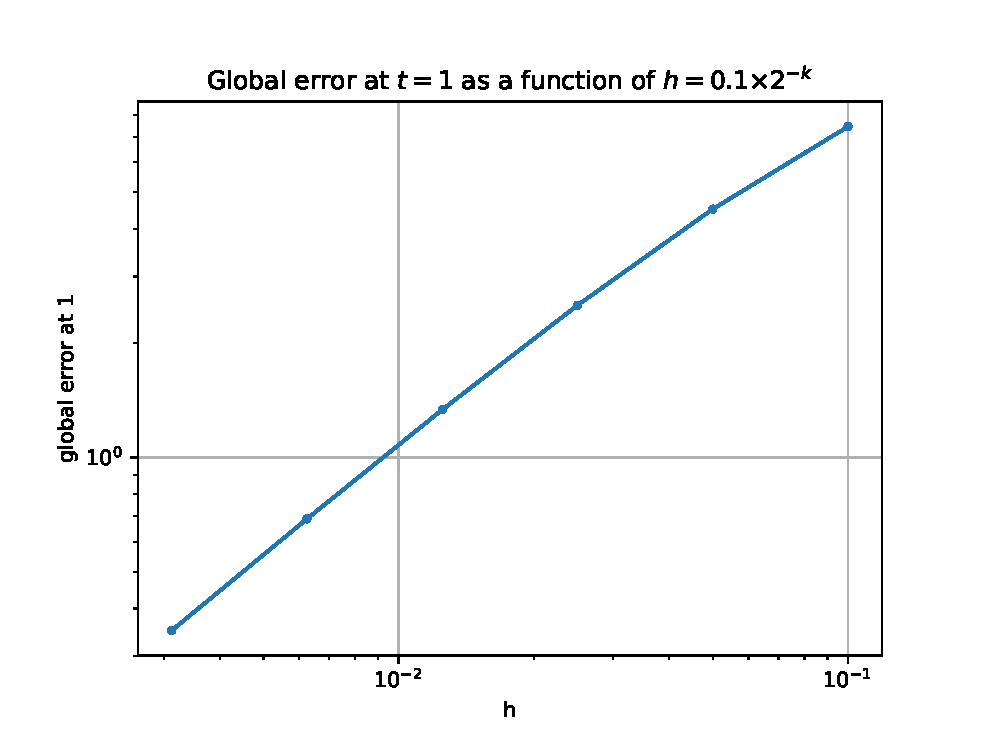
\includegraphics{plot31.eps}


%----PREGUNTA DOS -----
\noindent
\subsection{Trabajo, precisión y orden}
Consideremos otra vez el PVI (1), y su solución exacta, (2). En la tabla 2 comparamos
el error del método del trapecio con dos pasos distintos y de Runge-Kutta 4 (RK4). 

\begin{table}[h]
\caption{Comparación de RK4 y trapecio}
\centering
\begin{tabular}{cccc}
\hline \hline
$ $ & Trapecio($h_1$) & Trapecio($h_2$) & RK4 \\
Error global en $t=1$ & 0.7792153733  &  0.2218238872 & 0.0042700959 \\
Número de estados  &     20       &       40       &       40 \\
\hline
\end{tabular}
\end{table}
En este caso, es más conveniente cambiar a un método de mayor orden que reducir el
tamaño del paso. Tanto RK4 con paso $h_1$ como el método del trapecio con paso 
$h_2$ tienen cuarenta estados, pero el error con RK4 es significativamente menor.
Esto se debe a que en el método del trapecio, el error global es $O(h^2)$, así que al dividir el paso entre 2, reducimos el error por un factor de 4. En cambio, al 
cambiar a RK4, el error es $O(h^4)$, así que manteniendo  la misma h, reducimos el 
error global en un factor de (1/100)/(1/10000)=100, que es significativamente menor.

%---- PREGUNTA TRES ----
\noindent
\subsection{Método del punto medio}
Trabajaremos ahora en el intervalo [0,1] con el PVI 
\begin{align*}
\dot{y} = \begin{pmatrix}
-y_1+y_2 \\
-y_1-y_2
\end{pmatrix}
\ \ \ \ y(0) = \begin{pmatrix}
0  \\ 1
\end{pmatrix}
\end{align*}
Observemos que la solución exacta es 
\begin{align*}
y(t) = \begin{pmatrix}
e^{-t}\sin t\\
e^{-t} \cos t
\end{pmatrix}
\end{align*}
Usando el método del punto medio, con $h = \frac{1}{10}$ el error global en $t=1$ es  
0.0.00184835935056, mientras que con $h = \frac{1}{100}$ es $1.70989717275 \times 	
10^{-5}.$ Este error es consistente con la teoría, pues por ser de orden dos,
esperaríamos que al reducir el paso diez veces, el error se redujera cien (diez al 
cuadrado) veces; y dividiendo el primer error entre cien, obtenemos $1.84835935056
\times 10^{-5}$, muy cercano al experimental.


%---- PREGUNTA CUATRO ----
\noindent
\subsection{Ecuaciones \textit{stiff}}
Consideremos el PVI
\begin{align*}
\dot{y} = 5y-3y^2, \ \ y(0) = \frac{1}{2}, \ \ t \in [0,20]
\end{align*}
Observemos primero que las soluciones de equilibro de la ecuación son $y \equiv 0$ y 
$y \equiv \frac{5}{3}$.
Aplicando Euler implícito con paso constante $h = \frac{1}{2}$, obtenemos que
$y(20) \approx w_{20} = 1.\bar{6} = 5/3$, la solución de equilibrio hacia
la cual converge.
Aplicando Euler explícito con distintos pasos ($h \in \{\frac{1}{6}, \frac{1}{5}, 
\frac{1}{4}, \frac{1}{2} \}$) obtenemos convergencia a la misma solución en todas
excepto $h = \frac{1}{2}$, que aproxima $w_{20} = 2.04166028173897$.

Esto se debe a que la ecuación es \textit{stiff}, y para que la función de iteración
dada por el método de Euler explícito converja al punto fijo $w^* = \frac{5}{3}$, se
requiere $|F'(\frac{5}{3})| = |1+5h-6h\frac{5}{3}|<1$. Y esto se da si y sólo si 
$0 < h < \frac{2}{5}$. Por eso no funcionó cuando $h$ era 0.5.

Si ahora aplicamos el método de Bogacki–Shampine [Sa12]  con tolerancia $tol = 
\frac{1}{10}$  obtenemos $w_{20} = 1.6599026665708498$; y si bajamos la tolerancia 
hasta  $\frac{1}{100}$, aproximamos $w_{20} = 1.6851656759039848$.

De aquí, se puede ver que el método implícito es mejor que el método explícito 
adaptativo. Esto tiene una razón de ser. Para ajustar el paso del método de 
Bogacki-Shampine, se asume implícitamente que el error del método de menor orden 
es exactamente $h^3$, en vez de el verdadero $O(h^3)$. En la notación big-$O$, se 
esconde un factor que en la mayoría de los casos es pequeño. Sin embargo, en la 
ecuación presentada, al ser \textit{stiff}, tiene una tercera derivada con magnitud 
muy chica cerca de $y=\dfrac{5}{3}$, y mucho más grande cuando se aleja de este valor.

Por lo tanto, al reescalar $h$ usando $h_{nueva}=h_{vieja}\sqrt[3]{tol/error_{viejo}}$, 
nuestra $h$ nueva tendrá un error más grande que el previsto al asumir que el error es
$h^3$. Al dar múltiples pasos, el error se acumulará, y no será tan preciso como el 
incondicionalmente estable Euler implícito.
\end{document}
